\chapter{Design}
\label{chap:design}

\section{Overall Design}
\label{sec:overall_design}
The design of the GolfBot is centered around creating a robust and functional platform capable of navigating semi-structured outdoor environments while performing its specialized repair task. The system's design can be broken down into three core areas: the physical mechanical structure, the electronic hardware architecture, and the software architecture that governs its behavior. This chapter details the design decisions made in each of these areas. Figure \ref{fig:golfbot_system_diagram} provides a visual overview of the completed robot.

\begin{figure}[h!]
    \centering
    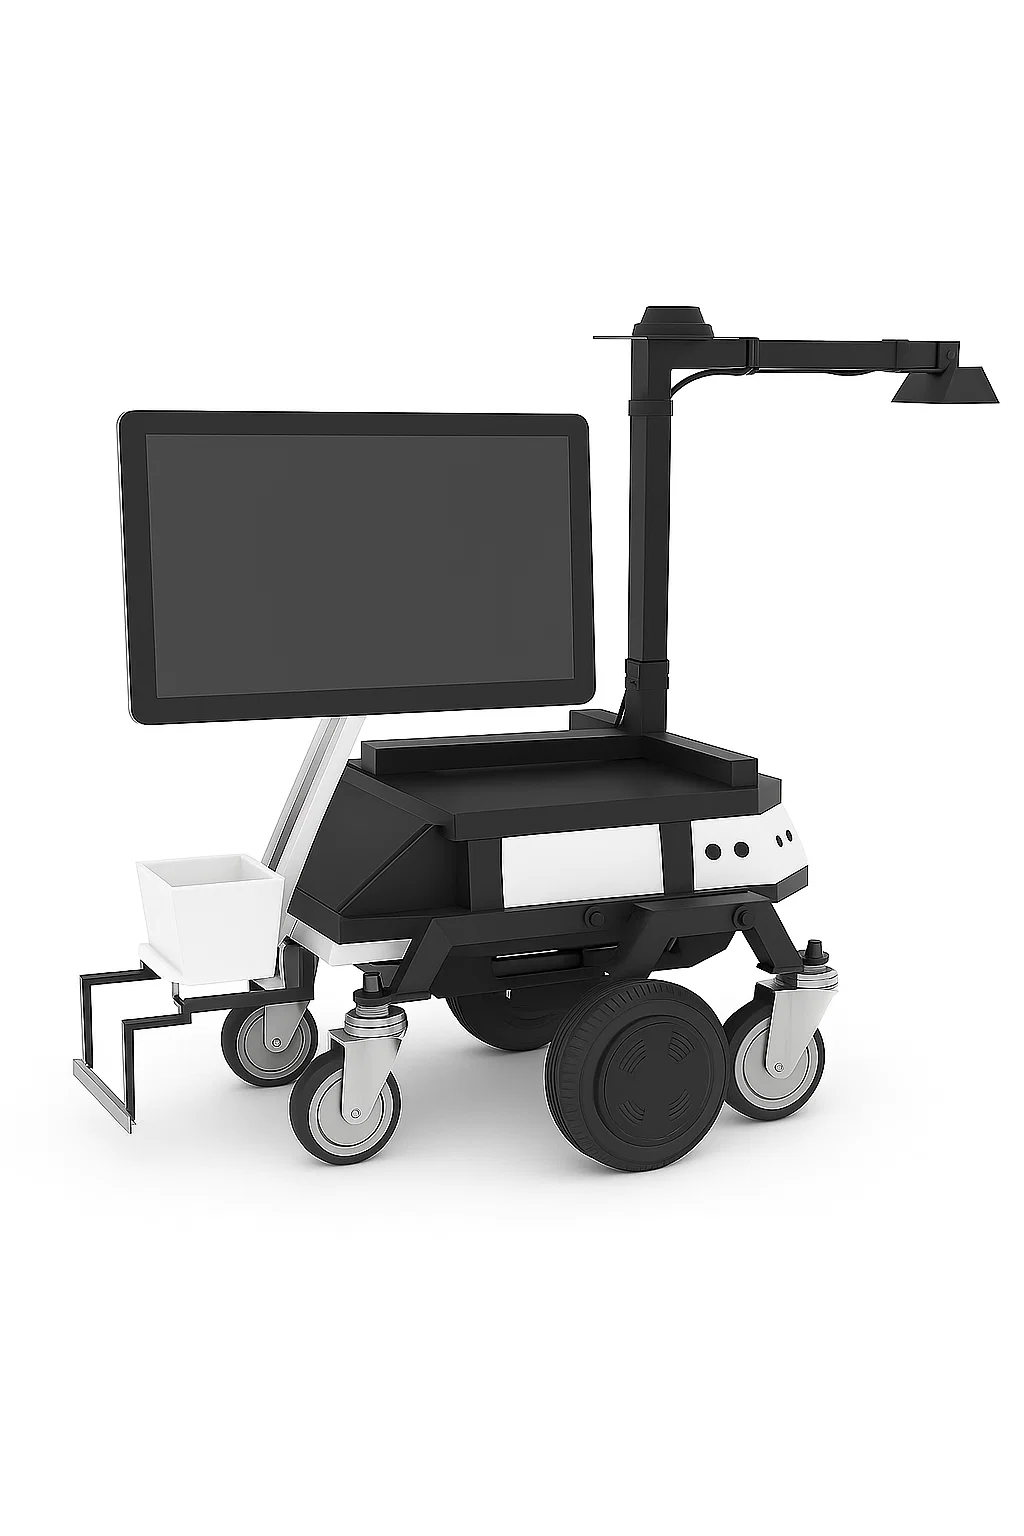
\includegraphics[width=0.7\linewidth]{figures/complete.png}
    \caption{GolfBot System Diagram}
    \label{fig:golfbot_system_diagram}
\end{figure}

\section{Mechanical Design}
\label{sec:mechanical_design}
The mechanical design focuses on the robot's physical construction, ensuring stability, durability, and the proper placement of all sensors and actuators.

\subsection{Chassis and Drivetrain}
\label{ssec:chassis_drivetrain}
The robot's structure is based on a lightweight aluminum chassis with main body dimensions of 500 mm x 360 mm x 115 mm. It uses a differential drive architecture, powered by two wheel hub motors with a wheel diameter of 165 mm and a track width (distance between the motors) of 570 mm. For stability, the drivetrain is supported by rubber caster wheels.

The motor hubs and casters are mounted on two swing arms, which function as a simple suspension system. This allows the robot's main body to remain relatively horizontal while the swing arms absorb minor bumps from uneven terrain. The wheels provide a ground clearance of 100 mm, sufficient for overcoming common obstacles on a golf course fairway. To protect the electronics, all internal components are housed within the main body frame, secured in custom 3D-printed holders and attached with strong, double-sided Velcro to prevent movement during operation.

\subsection{Sensor and Component Mounting}
\label{ssec:sensor_mounting}
To ensure optimal data collection, custom mounts were designed for the primary sensors. An L-shaped 25 mm aluminum box section is mounted on top of the robot's aluminum plate. This structure holds the camera 300 mm in front of the robot and 600 mm above the ground, providing a clear and effective field of view. To protect the camera from direct sunlight and physical impacts, it is housed in a 3D-printed holder featuring a 90-degree hinge, which ensures the camera is positioned orthogonally to the ground.

The same aluminum arm also supports a 2 mm thick stainless steel circular plate that serves as a ground plane for the RTK-GPS rover antenna. Additionally, a stand for the LCD screen, used for the graphical user interface, is mounted on the top frame.

\subsection{Dispensing and Repair Mechanism}
\label{ssec:dispenser_mechanism}
The repair system is mounted at the rear of the robot. A 90-degree folded stainless steel bracket, which was laser-cut for precision, holds the sand dispenser 100 mm above the ground and approximately 900 mm behind the camera's center point. The dispenser itself is 3D-printed from PLA plastic. Its core is a screw auger mechanism, powered by a NEMA 17 stepper motor, which pushes the sand-seed mixture from a hopper out through a nozzle.

Mounted directly behind the dispenser nozzle is a rubber-mounted brush. This brush extends 60 mm from the nozzle and serves to evenly spread the dispensed material, ensuring the divot is filled smoothly. It is attached to the same stainless steel bracket using custom 3D-printed mounts.

\subsection{RTK Base Station Design}
\label{ssec:rtk_base_design}
The ArduSimple RTK system requires a stationary base station to provide correction data to the rover. For this, the base module was placed inside a waterproof plastic box and mounted on a metal pipe. A circular, laser-cut metal plate is fixed to the top of the pipe to hold the RTK base antenna. To ensure signal integrity, this entire assembly is designed to remain stationary, positioned at the highest practical point within the robot's operational area. The base station is powered via a standard USB cable, which can be connected to a laptop or a simple USB wall adapter.

\section{Hardware Architecture}
\label{sec:hardware_architecture}
The hardware architecture describes the electronic components and the flow of data between them. It is designed around a central, powerful controller that processes sensor data and sends commands to the various actuators.

The Arduino Uno plays a critical role as a dedicated low-level controller. It is responsible for managing the NEMA 17 stepper motor (via the A4988 driver) for the dispensing mechanism and reading orientation data from the BNO055 IMU sensor. The Arduino communicates with the main Jetson Orin controller over a serial-over-USB connection. The Rover RTK-GPS module is also connected directly to the main controller via USB, providing it with high-precision location data. This separation of concerns allows the main controller to focus on high-level processing while the Arduino handles real-time actuator control and sensor reading.

\section{Software Architecture}
\label{sec:software_architecture}
% The software architecture of the GolfBot, detailing the ROS 2 nodes, topics, and overall data flow. This section will explain how the different software components (vision, navigation, control) interact.```
